\documentclass[twoside]{article}


\usepackage[T2A]{fontenc}                   %!? закрепляет внутреннюю кодировку LaTeX
\usepackage[utf8]{inputenc}                 %!  закрепляет кодировку utf8
\usepackage[russian,english]{babel}         %!  подключает русский и английский
\usepackage[margin=1.8cm]{geometry}         %!  фиксирует оступ на 2cm

\usepackage[unicode, pdftex]{hyperref}      %!  оглавление для панели навигации по PDF-документу + гиперссылки

\usepackage{amsthm}                         %!  newtheorem и их сквозная нумерация
\usepackage{hypcap}                         %?  адресация на картинку, а не на подпись к ней
\usepackage{caption}                        %-  позволяет корректировать caption 
\usepackage{fancyhdr}                       %   добавить верхний и нижний колонтитул
\usepackage{wrapfig}                        %!  обтекание таблиц и рисунков

\usepackage{amsmath}                        %!  |
\usepackage{amssymb,textcomp, esvect,esint} %!  |важно для формул 
\usepackage{amsfonts}                       %!  математические шрифты
\usepackage{mathrsfs}                       %  добавит красивые E, H, L
% \usepackage{ulem}                           %!  перечеркивание текста
\usepackage{abraces}                        %?  фигурные скобки сверху или снизу текста
\usepackage{pifont}                         %!  нужен для крестика
\usepackage{cancel}                         %!  аутентичное перечеркивание текста
\usepackage{esvect}                         %  добавит вектора стрелочками

\usepackage{graphicx}                       %?  графическое изменение текста
\usepackage{indentfirst}                    %   добавить indent перед первым параграфом
\usepackage{xcolor}                         %   добавляет цвета
\usepackage{enumitem}                       %!  задание макета перечня.

\usepackage{booktabs}                       %!  добавляет книжные линии в таблицы
% \usepackage{multirow}                       %   объединение ячеек в таблицах
% \usepackage{tikz}                           %!  высокоуровневые рисунки (кружочек)
% \usepackage{import}                         %   |
% \usepackage{xifthen}                        %   |
% \usepackage{pdfpages}                       %   | вставка рисунков pdf_tex
% \usepackage{transparent}                    %   |

\usepackage{bbm}                            %   добавляет \mathbbm{1}

% \newtheorem{to_thr}{Thr}[section]
% \newtheorem{to_suj}[to_thr]{Suj}
% \newtheorem{to_lem}[to_thr]{Lem}
% \newtheorem{to_com}[to_thr]{Com}
% \newtheorem{to_con}[to_thr]{Con}
% \theoremstyle{definition}
% \newtheorem{to_def}[to_thr]{Def}


\newenvironment{itemize*}
{
    \vspace{-\topsep}
    \begin{itemize}
        \setlength{\itemsep}{1pt}
        \setlength{\parskip}{1pt}
        }
    {\end{itemize}
}

\newenvironment{enumerate*}
{
    \vspace{-\topsep}
    \begin{enumerate}
        \setlength{\itemsep}{1pt}
        \setlength{\parskip}{1pt}}
    {\end{enumerate}
}

% \newenvironment{description*}
% {
%     \begin{description}
%         \setlength{\itemsep}{1pt}
%         \setlength{\parskip}{1pt}}
%     {\end{description}
% }

\definecolor{ugrey}{HTML}{666666}
% \definecolor{ublue}{HTML}{08088A}
% \definecolor{linkcolor}{HTML}{0000CC}
% \definecolor{urlcolor}{HTML}{006600}
% \hypersetup{
%     pdfstartview=FitH,  
%     linkcolor=linkcolor,
%     urlcolor=urlcolor, 
%     colorlinks=true,
%     citecolor=blue}
% базовая подстройка
\renewcommand{\d}{\, d}
\renewcommand{\leq}{\leqslant}
\renewcommand{\geq}{\geqslant}


% авторские команды
\newcommand{\vc}[1]{\boldsymbol{#1}}
\newcommand{\1}{\mathbbm{1}}
\newcommand{\T}{^{\textnormal{T}}}
\newcommand{\D}{^{\dag}}
\newcommand{\sub}[2]{#1_{\textnormal{#2}}}
\newcommand{\vp}{\vphantom{\dfrac{1}{2}}}
\newcommand{\hc}{\mathrm{h.c.}}

% операторы (просто прямой текст)
\renewcommand{\Im}{\mathop{\mathrm{Im}}\nolimits}
\renewcommand{\Re}{\mathop{\mathrm{Re}}\nolimits}
% \renewcommand{\P}{\mathop{\mathrm{P}}\nolimits}
% \newcommand{\E}{\mathop{\mathrm{E}}\nolimits}
% \newcommand{\D}{\mathop{\mathrm{D}}\nolimits}
% \newcommand{\cov}{\mathop{\mathrm{cov}}\nolimits}
\newcommand{\diag}{\mathop{\mathrm{diag}}\nolimits}
\newcommand{\std}{\mathop{\mathrm{std}}\nolimits}
\newcommand{\mean}{\mathop{\mathrm{mean}}\nolimits}
\newcommand{\sigmoid}{\mathop{\mathrm{sigmoid}}\nolimits}
\newcommand{\card}{\mathop{\mathrm{card}}\nolimits}
\newcommand{\grad}{\mathop{\mathrm{grad}}\nolimits}
\renewcommand{\div}{\mathop{\mathrm{div}}\nolimits}
\newcommand{\rot}{\mathop{\mathrm{rot}}\nolimits}
\newcommand{\Ker}{\mathop{\mathrm{ker}}\nolimits}
\newcommand{\spec}{\mathop{\mathrm{spec}}\nolimits}
\newcommand{\sign}{\mathop{\mathrm{sign}}\nolimits}
\newcommand{\tr}{\mathop{\mathrm{tr}}\nolimits}
\newcommand{\rg}{\mathop{\mathrm{rg}}\nolimits}
\newcommand{\const}{\textnormal{const}}


% цветной текст
\newcommand{\grey}[1]{\textcolor{ugrey}{#1}}
\newcommand{\red}[1]{\textcolor{red}{#1}}
\newcommand{\green}[1]{\textcolor{urlcolor}{#1}}
\newcommand{\blue}[1]{\textcolor{ublue}{#1}}


% символы
\newcommand{\cmark}{\text{\ding{51}}}
\newcommand{\xmark}{\text{\ding{55}}}


% подгрузка pdf_tex картинок
% \newcommand{\incfig}[1]{%
%     \def\svgwidth{\columnwidth}
%     \import{./figures/}{#1.pdf_tex}
% }

\newcommand{\addletter}[2]{\begin{picture}(7,7) \put(0,#1){{#2)}} \end{picture}}



% специфично к квантам
\newcommand{\ket}[1]{\left| #1 \right\rangle}
\newcommand{\bra}[1]{\left\langle #1 \right|}

% \newcommand{\dppp}{\frac{d^3 p}{(2 \pi \hbar)^3}}

\DeclareDocumentCommand{\bk}{m o m}{
    \IfNoValueTF{#2}{\langle #1 | #3 \rangle}{\langle #1 | #2 | #3 \rangle}
}
\newcommand{\kb}[2]{| #1 \rangle \langle #2 |}

\newcommand{\tth}{\sub{t}{th}}
% !TEX root = ../master-thesis.tex

% add page header

\pagestyle{fancy}
\fancyhf{}
% \fancyhead[RE,LO]{\thepage}
% \fancyhead[LE,RO]{Ж\raisebox{-1.5pt}{и}К}
% \fancyhead[CO,CE]{\nouppercase{\textit{\leftmark}}}
\fancyhead[LE,RO]{\nouppercase{\textit{\leftmark}}}
\fancyfoot[LE,RO]{\thepage}




\DeclareRobustCommand{\tmpsim}{ %%%%%%%%%%%%%% ~ < %%%%%%%%%%%%%%%%%%%
  \mathbin{\text{
      \raisebox{-1pt}{
            \hspace{-4.5pt} \rotatebox{-26}{\scalebox{0.8}[0.7]{$\sim$}}
        }
  }}
}
\def\lesim{{
    \setbox0\hbox{$\ <\ $}
    \rlap{\hbox to \wd0{\hss$\tmpsim$\hss}}\box0
}}
%%%%%%%%%%%%%%%%%%%%%%%%%%%%%%%%%%%%%%%%%%%%%%%%%%%%%%%%%%%%%%%%%%%%%%


\def\letuscom{%%%%%%%%%%%%%%%%%%%%%% ПУСТЬ %%%%%%%%%%%%%%%%%%%%%%%%%%
\mathord{\setbox0=\hbox{$\exists$}%
     \hbox{\kern 0.125\wd0%
           \vbox to \ht0{%
              \hrule width 0.75\wd0%
              \vfill%
              \hrule width 0.75\wd0}%
           \vrule height \ht0%
           \kern 0.125\wd0}%
   }%
}
\newcommand{\letus}{\raisebox{-1.2pt}{$\letuscom$}}
%%%%%%%%%%%%%%%%%%%%%%%%%%%%%%%%%%%%%%%%%%%%%%%%%%%%%%%%%%%%%%%%%%%%%%


\usepackage{arydshln} %%%%%%%%%%%%%%% ЛИНИИ В МАТРИЧКЕ %%%%%%%%%%%%%%%
\makeatletter
  \renewcommand*\env@matrix[1][*\c@MaxMatrixCols c]{%
    \hskip -\arraycolsep
    \let\@ifnextchar\new@ifnextchar
  \array{#1}}
\makeatother
%%%%%%%%%%%%%%%%%%%%%%%%%%%%%%%%%%%%%%%%%%%%%%%%%%%%%%%%%%%%%%%%%%%%%%


\makeatletter %%%%%%%%%%%%%%% КРУЖОЧЕК %%%%%%%%%%%%%%%%%%%%%%%%%%%%%%%
\newcommand*{\encircled}[1]{\relax\ifmmode\mathpalette
\@encircled@math{#1}\else\@encircled{#1}\fi}
\newcommand*{\@encircled@math}[2]{\@encircled{$\m@th#1#2$}}
\newcommand*{\@encircled}[1]{%
  \tikz[baseline,anchor=base]{\node[draw,circle,outer sep=0pt,
                                        inner sep=.2ex] {#1};}}
\makeatother
%%%%%%%%%%%%%%%%%%%%%%%%%%%%%%%%%%%%%%%%%%%%%%%%%%%%%%%%%%%%%%%%%%%%%%




\begin{document}

% set skip of equation length 

\setlength{\abovedisplayskip}{3pt}
\setlength{\abovedisplayshortskip}{3pt}
\setlength{\belowdisplayskip}{3pt}
\setlength{\belowdisplayshortskip}{3pt}
\setlength{\headheight}{13pt}

% \numberwithin{equation}{section}

% \renewcommand{\thesubsection}{\thesection.\alph{subsection}}





% document's head

\begin{center}
    \LARGE \textsc{Fermionic State Preparation and Imaging \\ in Optical Tweezer Array}
\end{center}

\hrule

\phantom{42}

\begin{flushright}
    \begin{tabular}{rr}
        % \textbf{Author}: 
        & Khoruzhii Kirill \\
        % & \\
    % date:
        % \textbf{Date}:
        & \textit{Munich, \today}\\
    \end{tabular}
\end{flushright}

\noindent
Quantum simulation with ultracold atoms requires both high-fidelity preparation of the initial many-body state and site-resolved measurement of the final state. This thesis presents the development of experimental techniques for spin-resolved free-space imaging and deterministic, spin-selective preparation of ultracold fermionic $^6$Li atoms in a two-dimensional optical tweezer array. The array is generated using crossed acousto-optic deflectors, with precise control achieved through a combination of direct camera-based calibration and atom-based feedback. A novel spilling method enables the preparation of arbitrary spin- and site-resolved occupation patterns. The thesis also introduces numerical tools for simulating Fermi-Hubbard dynamics in small systems, laying the groundwork for future out-of-equilibrium quantum simulation experiments.







\thispagestyle{empty}

\tableofcontents

% \vfill

% Базовая структура диплома:
% \begin{enumerate*}
%     \item deterministic state preparation (single tweezer)
%     \begin{enumerate*}
%         \item loading (2D MOT, MOT, Dipol Trap, Tweezer)
%         \item spilling
%     \end{enumerate*}
%     \item single-atom spin resolved free space imaging
%     \begin{enumerate*}
%         \item ! flashing and model
%         \item ! image processing
%     \end{enumerate*}
%     \item deterministic state preparation (tweezer array)
%     \begin{enumerate*}
%         \item ! generating
%         \item ! control
%         \item ! balancing
%     \end{enumerate*}
% \end{enumerate*}

% Это история про то как сделать и сфотографировать спиновое состояние в твизере.   

% Нужно выписать contributions! И им следовать.   




\newpage


 
Ещё было бы здорово добавить картинки

\begin{itemize}
	\item Демонстрация с Random Unitaries (Xinyi тезис)
	\item Схема установки, фото 3D mot
	\item BEC
	\item ? Feshbach resonance
	\item Imaging: Эксперимент. Alternating beams (с осциллографа), разница двух облачков (один, два continous, два alternating)
	\item Imaging: histogram noise vs atoms, raw nuvu img
	\item MWM (simulation, ? observed)
	\item Flashing. Экспериментальная установка, табличка с её параметрами
	\item State preparation: spilling. Схематичное изображение (посмотреть в Heidelberg thesis). Step plot. 
	\item State preparation: схема подготовки site- and spin- resolved состояния.
	\item Стабилизация: итерации стабилизации для single-value feedback
	\item Theory: описание fermi-hubbard, фазовая диаграмма (посмотреть coepsill)
	\item Theory: термализация vs локализация для решётки 8x8
	\item Theory: вклад от лабиринтов в локализацию
	\item Tweezer Array. Схема AOD, crosstalk basics
\end{itemize}



\section{Single-atom spin resolved free space imaging}

\subsection{Experimental setup}
\red{Здесь схема оптики для подготовки лучей в preparation board и схема лучей и подключения для main board}.

\begin{figure}
    \centering
    \addletter{140}{a}
    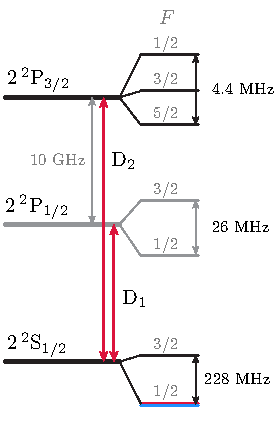
\includegraphics{fig-ai/li-levels-base.pdf}
    \hfill
    \addletter{140}{b}
    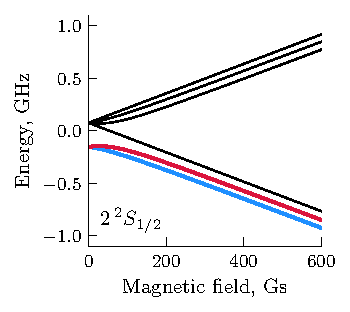
\includegraphics{fig-py/li6-zeeman.pdf}
    \hfill
    \addletter{140}{c}
    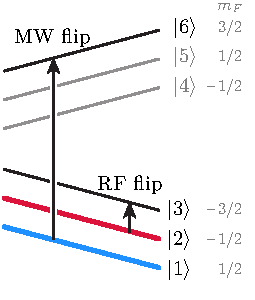
\includegraphics{fig-ai/li-levels.pdf}
    \caption{
        \textbf{${}^6$Li energy levels}. 
        a) Level diagram of the ground and 2P excited states of ${}^6$Li \cite{gehm_preparation_2003}. 
        b) Zeeman splitting of the hyperfine levels of the $2\, {}^2\mathrm{S}_{1/2}$ state in ${}^6$Li \cite{serwane_deterministic_2011, sibalic_arc_2017}. With dashed line was marked non-interacting regime for 1-2 mixture at 527 Gs. c) As different spin states for physics we consider state $\ket{1}$ and $\ket{2}$, but for imaging it is worth to flip them to close transitions.
        \red{Можно разделить (b), чтобы показать и расщепление для P32.}
    }
    \label{fig:li6levels}
\end{figure}

\subsection{SSH Model}
Исходно SSH model выглядит как
\begin{equation*}
	H = t_1 \sum_n \kb{n,B}{n,A} + t_2 \sum_n \kb{n+1, A}{n, B} + \hc
\end{equation*}
что в нашем случае переписывается в виде
\begin{equation*}
	H = \frac{\Omega_1}{2} \sum_p \kb{p,g}{p+1,e} + \frac{\Omega_2}{2} \sum_p \kb{p-1,e}{p,g} + \hc
\end{equation*}
где в случае с flashing коэффициенты становятся зависимыми от времени. Можно численно решить уравнение Линдблада для TLS в двух случаях
\begin{equation*}
	i \hbar \partial_t \rho = [H, \rho] + \mathcal{L}[\rho]
\end{equation*}


Таким образом принципиально делать лучи чередующимеся. Тут можно добавить картинку $\rho(t, k)$ (done) и схемы с ssh моделью и тем как лучи используем. 






\begin{figure}
    \centering
    \addletter{140}{a}
    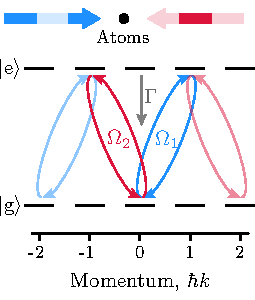
\includegraphics{fig-ai/ssh-scheme.pdf}
    \hfill
    \addletter{140}{b}
    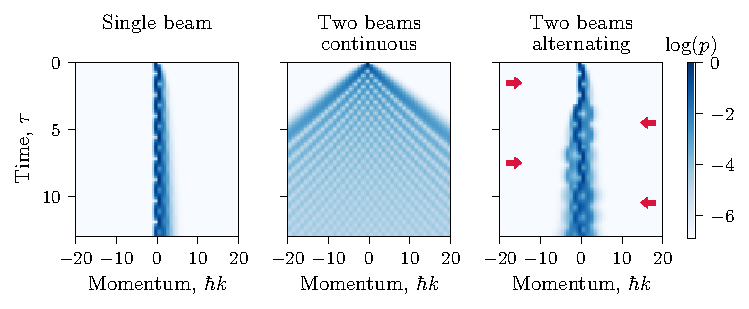
\includegraphics{fig-py/ssh-model.pdf}
    \caption{
        \textbf{Momentum-space dynamics in the SSH model}. 
        a) Atoms undergo momentum-changing transitions via couplings $\Omega_1$ and $\Omega_2$, realizing a SSH-like quantum walk.
        b) Momentum distributions over time for different beam configurations: single beam (left) shows small shift; two continuous beams (middle) result in fast spreading; alternating beams (right) suppress spread.
    }
    \label{fig:sshmodel}
\end{figure}











\subsection{Image Processing}
На каждой из фотографий в каждой выделенной области хочется уметь отличать наличие атома от его отсутствия, что в контексте наличия шумов становится нетривиальным. Можно было бы просто посчитать Pixel Integral \red{(добавить рисунок, а)}, но можно лучше. Расположим оптику (схема оптики) таким образом, что в среднем на пиксель приходилось по фотону. \red{Измерим} какой сигнал на один фотон мы ожидаем и в соответсвии с этим выставим threshold. Таким образом может быть отфильтрована большая часть шума \red{(b)}. Но дальше можно воспользоваться информацией о том, что атомы излучают кучно \red{(пример двух фото с одним counts, с атомом и без)}, в отличие от случайного шума. Так что отфильтровав низкие частоты, свернув изображение с гауссовым фильтром, пролучаем \red{(c)}. 


















\section{Tweezer Array}

\subsection{Experimental setup}
\red{Здесь схема оптики для подготовки лучей твизеров, схема подключения и генерации}.




\subsection{Generating with AODs}
...


% \textbf{Acousto Optic Deflector (AOD)}. AOD, как и AOM, состоит из кристалла, который модулируется пьезоэлементом. Проходящие через кристалл фотоны $(\sub{\vc{k}}{in}, \sub{\omega}{in})$ рассеиваются на фононах $(\vc{q}, \Omega)$ via Bragg diffraction. To have higher efficiency we need to satisfy Bragg condition (проверить и добавить источник)
% \begin{equation*}
% 	\sub{n}{sc} q = \sub{k}{in} \sin(\theta),
% \end{equation*}
% \grey{где $\theta$ это угол между $\vc{k}$ и нормалью к $\vc{q}$} \red{(добавить рисунок)}. Внутри AOD находится несколько пьезоэлементов, к которым ведут провода подобранной длины так, чтобы при изменение частоты $\Omega$ направление $\vc{q}$ менялось соответсвующим Bragg condition образом. Это помогает улучшить диффракционную эффективность \grey{(добавить определение или ссылку)} AOD. На выходе полуются $(\sub{\vc{k}}{out}, \sub{\omega}{out}) = (\sub{\vc{k}}{in}+\vc{q}, \sub{\omega}{in} + \Omega)$. 
% Имея набор частот в модулирующем сигнале $(\vc{q}_j, \Omega_j)$ получим на выходе набор лучей
% \begin{equation*}
% 	(p_j, \vc{k}_j, \omega_j) = (F_j(\vc{a}, \sub{\vc{\omega}}{in}), \sub{\vc{k}}{in}+\vc{q}_j, \sub{\omega}{in} + \Omega_j),
% \end{equation*}
% c мощностью в каждом луче на выходе $p_j$. Регулируя вектор амплитуд $\vc{a}$, подающихся в AOD можно контролировать выходную мощность $\vc{p}$. 


\subsection{Control}
% !TEX root = ../master-thesis.tex

\textbf{Frequency to position mapping.}
To extract the local intensities $P_{ij}$ from camera images, we need to determine which pixels correspond to which tweezer sites. For this purpose, we define an affine transformation from the drive frequency space $(\omega_{\mathrm{hor}}, \omega_{\mathrm{ver}})$ to image plane coordinates $(x, y)$:
\begin{equation*}
    \vc{r} = H \vc{\omega},
    \hspace{5 mm} \Leftrightarrow \hspace{5 mm} 
    \begin{pmatrix}
        x \\ y
    \end{pmatrix} = \begin{pmatrix}
        h_{11} & h_{12} & h_{13} \\
        h_{21} & h_{22} & h_{23}
    \end{pmatrix} 
    \begin{pmatrix}
        \sub{\omega}{hor} \\
        \sub{\omega}{ver} \\
        1
    \end{pmatrix}.
\end{equation*}
Here, $H$ is a $2 \times 3$ matrix calibrated from a set of measured spot positions. For example, one can measure $\vc{r}_j$ for random frequency vectors $\vc{\omega}_j \in [\omega_{\mathrm{min}},\, \omega_{\mathrm{max}}]$, construct the matrices $\omega_{ij}$ with $i \in \{\mathrm{hor}, \mathrm{ver}\}$ and $r_{ij}$ with $i \in \{x, y\}$, and solve the least-squares problem:
\begin{equation}
    r = H \omega,
    \hspace{0.5cm} \Rightarrow \hspace{0.5cm}
    r \omega^\mathrm{T} = H \omega \omega^\mathrm{T}
    \hspace{0.5cm} \Rightarrow \hspace{0.5cm}
    r \omega^\mathrm{T} \left(\omega \omega^\mathrm{T}\right)^{-1} = H.
    \label{eq:linreg-freq2pos}
\end{equation}

This transformation defines a region of interest around each tweezer, within which we compute the integrated pixel intensity after background subtraction. The resulting values are proportional to the optical powers $P_{ij}$.

\textbf{Linear reconstruction.}
The mapping from input amplitudes $\vc{a}$ to optical power is approximated by Eq.~\eqref{eq:taylerexp}. In the regime $a_i \in [0.85, 0.95]$, a linear approximation is sufficient\footnote{
    For wider amplitude ranges, higher-order terms can be added to the model. However, this is unnecessary in the present context.
}. We construct the Jacobian matrix $F'_{ji}$ by fitting a linear regression model to a dataset of amplitude–intensity pairs. The resulting crosstalk matrix is shown in Fig.~\ref{fig:control}b. It is approximately diagonal, with comparable diagonal entries and off-diagonal elements typically reaching up to 30\% in magnitude relative to the diagonal, due to power redistribution between neighboring tones. Crosstalk between the horizontal and vertical AODs remains negligible.

The quality of the linear fit for the $4 \times 4$ array is illustrated in Fig.~\ref{fig:control}e. The total intensity (Fig.~\ref{fig:control}d) scales linearly with the average input amplitude, yielding $R^2 > 0.99$. Relative residuals are normally distributed with width $0.3\%$, confirming the applicability of the model in this range.

\textbf{Power-aware optimization.}
\grey{In the presence of limited laser power and finite AOM diffraction efficiency, we prefer solutions where all amplitudes remain close to 1. This preference can be incorporated into the optimization objective. In addition to minimizing intensity imbalance, we penalize deviations of the average amplitudes from a target value (e.g., 0.9).}



\begin{figure}
    \centering
    \addletter{170}{a}
    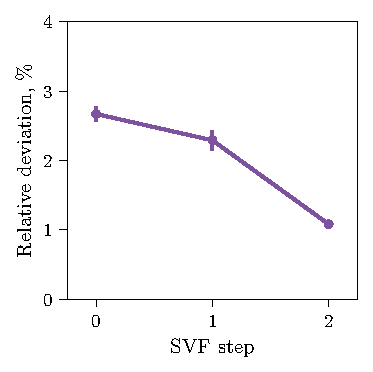
\includegraphics{fig-py/svf-avg.pdf}
    \addletter{170}{b}
    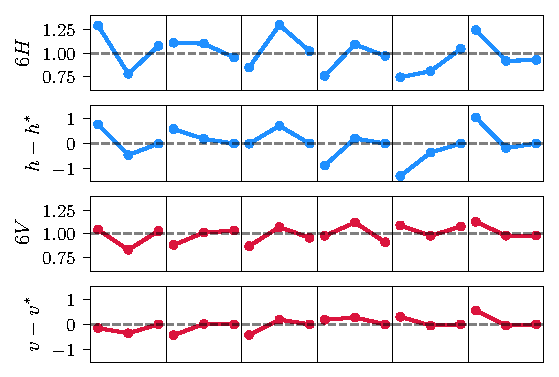
\includegraphics{fig-py/svf.pdf}
    \caption{
        \textbf{Single-value feedback (SVF) optimization for a $6 \times 6$ tweezer array.}
        (a) Relative deviation of effective powers $P_j$ across the array during successive SVF steps, quantified as $\mathrm{std}(P_j)/\langle P_j \rangle$. The initial point corresponds to camera-based balancing; subsequent iterations apply SVF with feedback rates $\gamma = 1/20$ and $\gamma = 1/40$. Further iterations did not yield statistically significant improvements. 
        (b) Retrieved horizontal powers $H_i$ and vertical powers $V_j$ (top and third rows), along with corresponding deviations of driving amplitudes from their final target values, $h - h^*$ and $v - v^*$. The recovered $H$, $V$ vectors are extracted from the photon count matrix $M_{ij}$ using factorization as described in \eqref{uv-decomposition}.
    }
    \label{fig:svf}
\end{figure}

\subsection{Balancing}
% !TEX root = ../master-thesis.tex



\grey{It is also possible to calibrate each AOD independently, without relying on an SVD-based approach. This alternative was not tested in the scope of this work. However, it is worth emphasizing that the SVD-based method is guaranteed to work even for double-AOD configurations~[ref], where crosstalk between the two directions can be significantly stronger.}

Precise control over the depth of each optical tweezer is essential for preparing few-fermion systems via spilling techniques. In our setup, each tweezer is initially loaded with approximately \red{100} atoms, which are then selectively removed by ramping down the potential depth. The number of remaining atoms as a function of spill power $x_{\mathrm{sp}}$ exhibits a quantized staircase structure, reflecting the discrete energy levels of the 1D harmonic oscillator. This behavior can be characterized by a step plot~\cite{holten_pauli_2022}.

\textbf{Step plot.}
To characterize this behavior in our tweezer array, we measure step plots for all sites simultaneously. Figure~\ref{fig:stepplot}a shows the result for a $4 \times 4$ array. For each value of $x_{\mathrm{sp}}$, we acquire 70 experimental realizations and compute the average photon signal per site. 
% This signal serves as a robust proxy for atom number. In contrast to single-atom counting, this approach is parameter-free and effective even for large initial occupancies.

\textbf{Uniformity characterization.}
To quantify depth inhomogeneity across the array, we fit each step trace with a sigmoid function:
\begin{equation*}
    \sigmoid(x) = \frac{A_j}{1 + \exp\left(-(x - x_j)/\sigma_j\right)},
\end{equation*}
where $x_j$ denotes the center of the step and $\sigma_j$ its width for tweezer $j$. We define a relative uniformity metric as $\std(x_j) / \langle x_j \rangle$. After camera-based balancing (Sec.~\ref{subsec:control}), this metric typically yields $\sim 3\%$, which is insufficient for deterministic preparation across the array. A more precise balancing procedure is therefore required.




\textbf{Single-value feedback.}
To further improve uniformity, we apply an iterative atom-based feedback scheme. Rather than fitting full step plots, we operate at a single point on the slope of the transition, near the half-filling level $A_j / 2$. At this point, the sigmoid can be approximated by a linear response:
\begin{equation*}
    \sigmoid(x) \approx \frac{A_j}{4 \sigma_j} x - \frac{A_j x_j}{4 \sigma_j},
\end{equation*}
assuming $x_j \gg \sigma_j$.  In the feedback loop, we do not use the fitted sigmoid parameters directly. Instead, we measure a single photon-count matrix $M_{ij}$ and treat it as a linear proxy for the power matrix $P_{ij}$. Since the sigmoid offset $\mathrm{shift} = A_j x_j / (4 \sigma_j)$ is known from the fits, we approximate:
\begin{equation}
    \label{mp-propto}
    M_{ij} + \mathrm{shift} \propto P_{ij} = \Lambda H_i V_j.
\end{equation}
We then factorize this matrix using the method introduced in \eqref{uv-decomposition} and update the amplitudes according to:
\begin{equation*}
    h \rightarrow h + \gamma (H - H_0), \qquad
    v \rightarrow v + \gamma (V - V_0),
\end{equation*}
where $(H_0, V_0)$ is the target point, and $\gamma$ is the feedback rate. This model-free procedure avoids full sigmoid fitting and operates directly on experimental measurements.

Figure~\ref{fig:stepplot}b shows the result of applying this single-value feedback (SVF) protocol to a $4 \times 4$ array. After five iterations, the relative deviation of the fitted step centers is reduced to $0.7(2)\%$, well within the plateau width (typically $\pm5\%$), enabling deterministic state preparation across the full array. \red{Add fig. with single value feedback progress.}

Figure~\ref{fig:svf}a shows the process of applying the SVF protocol to a $6 \times 6$ array. The proportionality coefficient in \eqref{mp-propto} is $A/4\sigma \sim 10(1)$ (the average value is chosen for the plot) for our experiment.

\subsection{State preparation}
% !TEX root = ../master-thesis.tex

% Тут хочется добавить общую последовательность эксперимента. То есть если говорю про imaging with flashing, добавим что происходит с магнитным полем и прочим важным (спросить Намана). Аналогично для state preparation, imaging.

% m: 40-42, 67-70
% h: 84-86, 


\begin{figure}
    \centering
    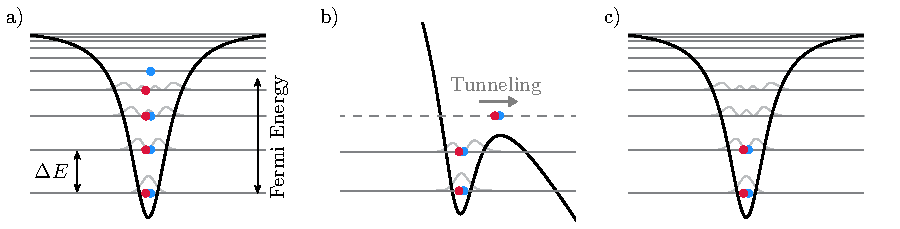
\includegraphics{fig-ai/preparation.pdf}
    \caption{
        \textbf{Deterministic preparation via spilling.}
        (a) Fermionic atoms are initially loaded into a tightly confined optical tweezer, forming a Fermi sea occupying the approximately 1D harmonic oscillator levels up to the Fermi energy. 
        (b) A magnetic field gradient tilts the potential, and the trap depth is lowered such that atoms above a defined spill level tunnel out. 
        (c) This procedure leaves a well-defined number of atoms in the lowest energy states, with a preparation fidelity of approximately 95\%. 
        Blue and red dots denote atoms in different spin states; gray curves indicate the bound-state wavefunctions.
    }
    \label{fig:preparation}
\end{figure}



\textbf{Tweezer loading.} We begin by preparing a spin-balanced mixture in the two lowest hyperfine states, $|1\rangle$ and $|2\rangle$, using a compressed magneto-optical trap (MOT). The atoms are initially loaded into a crossed ODT, where we perform evaporative cooling. This follows closely the sequence described in~\cite{culemann_construction_2024}.

After cooling, the atoms are transferred into a tightly focused optical tweezer potential. The loading process relies on the so-called \emph{dimple trick}~\cite{zurn_few-fermion_2012}, where a tightly confined but deep tweezer potential is superimposed onto the wider ODT reservoir. Because the tweezer affects only a small region of the total cloud, the global temperature $T$ remains approximately unchanged, while the local chemical potential is enhanced. In this regime, the average occupation number $\bar{n}(E_i)$ of a single-particle state $i$ with energy $E_i$ follows the Fermi-Dirac distribution:
\begin{equation}
    \bar{n}(E_i) = \frac{1}{e^{(E_i - \mu)/k_B T} + 1}.
\end{equation}
If the energy gap between the ground state $E_0$ and the Fermi energy $E_F$ is increased such that $(E_0 - E_F) / k_B \gg T$, then $\bar{n}(E_0) \rightarrow 1$. This ensures near-unity occupation of the lowest level, which provides an ideal starting point for deterministic preparation. In our experiment, this condition is achieved by ramping on the tweezer adiabatically while continuing evaporation inside the tweezer. The full loading and cooling sequence is depicted in Fig.~\ref{fig:preparationseq}.

\textbf{Deterministic few-body preparation via spilling.} To isolate a well-defined number of atoms in the lowest motional states of the tweezer, we use the \emph{spilling technique}, as described in~\cite{zurn_few-fermion_2012, holten_pauli_2022}. This method relies on tilting the potential with a magnetic field gradient and reducing the trap depth to allow atoms above a threshold energy to tunnel out. 
The resulting states are shown in Fig.~\ref{fig:preparation}. \red{See Appendix for details.}
% The energy levels and wavefunctions of the effective 1D potential under combined optical and magnetic fields were obtained numerically using a finite-difference method and the Thomas algorithm.

The spilling sequence is performed at a magnetic field of 527\,G, where the two spin states are nearly non-interacting. A magnetic field gradient of 20\,G/cm creates a linear tilt, and the tweezer power is lowered to a value that sets the spill threshold. After a short tunneling time, the trap depth is ramped back up to recapture the remaining atoms. By empirically optimizing these parameters, we achieve deterministic preparation of two atoms per tweezer with a fidelity of approximately 95\,\%. This sequence results in high-fidelity preparation within a total experimental cycle time of less than 2\,s.

% Стоит сказать, что система достаточно симметрична по отношению к уменьшению tweezer depth во время spilling или увеличению градиента. 


\begin{figure}
    \centering
    \addletter{140}{a}
    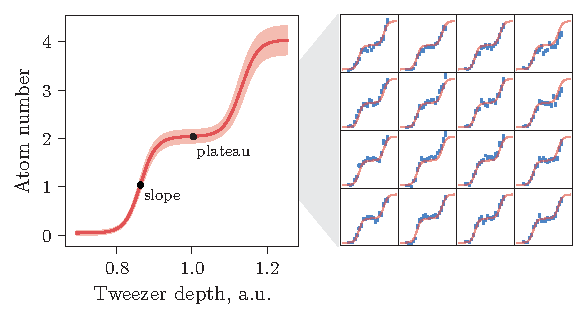
\includegraphics{fig-ai/step-plot-joined.pdf}
    \phantom{42}
    \addletter{140}{b}
    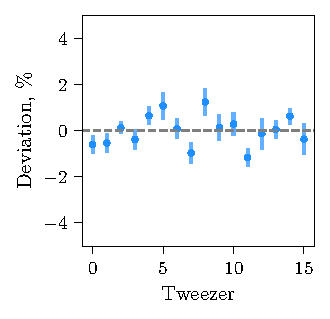
\includegraphics{fig-py/step-plot-balance.pdf} % 0.6 +- 0.2
    % 
    % 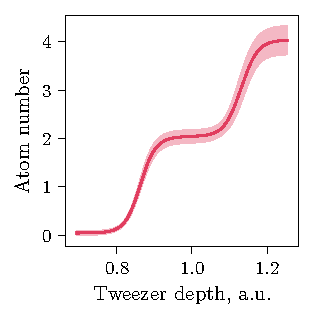
\includegraphics{fig-py/step-plot.pdf}
    % 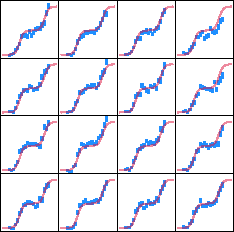
\includegraphics{fig-py/step-plot-inset.pdf}
    \caption{
        \textbf{Step plot.}
        (a) 
        Atom number as a function of tweezer depth during the spilling sequence. 
        % Plateaus correspond to quantized energy levels of the 1D harmonic oscillator. 
        Step plots for each tweezer in the $4 \times 4$ array are shown on the right. The average fit is shown as a solid red line, with standard deviation across sites indicated by the shaded area. 
        (b) Relative deviation of the fitted sigmoid centers for each tweezer after SVF balancing. The standard deviation is $0.7(2)\%$, which is well within the plateau width ($\pm 5\,\%$), ensuring sufficient uniformity for array-wide spilling. \red{$\chi^2$?}
        % All measurements were performed in this work using atom-based measurements and SVF-balanced tweezer depths.
    }
    \label{fig:stepplot}
\end{figure}



\section{Fermi-Hubbard Model}

\subsection{Introduction}
% !TEX root = ../master-thesis.tex

% --------------------------------------------------------------------------------------
% Intro
% --------------------------------------------------------------------------------------

% \textbf{Overview.}
Understanding the dynamics of isolated quantum systems remains one of the central goals of contemporary many-body physics. Over the last decades, considerable progress has been made in classifying and probing different dynamical regimes, from thermalizing phases consistent with conventional statistical mechanics to exotic non-ergodic phases that violate the Eigenstate Thermalization Hypothesis (ETH). Among these, the Fermi-Hubbard model has emerged as a paradigmatic platform for studying the interplay of interactions, quantum statistics, and disorder in strongly correlated systems.

In the clean, disorder-free limit, the Fermi-Hubbard model exhibits rich equilibrium physics, including Mott insulators, spin ordering, and pseudogap phenomena relevant to high-temperature superconductivity \cite{esslinger_fermi-hubbard_2010}. However, the model also serves as a fertile ground for exploring nonequilibrium phenomena, such as quantum quenches, relaxation, transport, and entanglement dynamics — especially when generalized to include disorder or spatial inhomogeneities.

Recently, theoretical and experimental attention has increasingly shifted toward the role of disorder in quantum many-body dynamics. It is now understood that disorder can lead to fundamentally different behaviors depending on the presence or absence of interactions. For instance:
\begin{itemize}
	\item In the absence of interactions, disorder induces \textit{Anderson localization}, which prevents particle diffusion and leads to persistent memory of initial conditions \cite{anderson_absence_1958}.
	\item When interactions are present, the system may enter the regime of \textit{many-body localization (MBL)}, characterized by the absence of thermalization and slow unbounded entanglement growth \cite{basko_metalinsulator_2006,nandkishore_many-body_2015}.
	% , and emergent local integrals of motion
	\item In contrast, when disorder is weak or absent, the system typically evolves toward local thermal equilibrium, consistent with the predictions of \textit{ETH} \cite{deutsch_quantum_1991,srednicki_chaos_1994}. 
\end{itemize}

These dynamical phases (\emph{thermal, Anderson-localized, and MBL}) are typically distinguished through the behavior of local observables, spectral statistics, and the dynamics of quantum correlations. Their interplay is especially rich in two dimensions, where the presence of more complex geometry, potential mobility edges, and rare-region effects make the dynamical phase diagram both challenging and intriguing.

From an experimental standpoint, studying such phenomena requires precise control over initial states, evolution Hamiltonians, and high-fidelity measurements of observables at the single-site level. This thesis presents a platform that provides such control, combining deterministic initialization of fermionic states in a two-dimensional tweezer array with programmable evolution under the Fermi-Hubbard Hamiltonian and spin- and site-resolved imaging.

Compared to conventional optical lattice experiments, the tweezer-based approach offers several key advantages for nonequilibrium quantum simulation:
\begin{enumerate}
	\item \textit{Deterministic and programmable state preparation.} Using a sequence of global and spin-selective spilling operations, arbitrary configurations of fermionic atoms can be prepared with high fidelity. This capability enables initialization of tailored many-body states for probing specific dynamical scenarios, such as local quenches, domain-wall melting, or imbalance relaxation.
	\item \textit{Fast experimental cycle and large statistics.} The entire experimental sequence, including preparation, evolution, and measurement, completes in under two seconds, allowing up to $10^5$ experimental repetitions per day. This rapid repetition rate is crucial for averaging over disorder realizations and collecting sufficient statistics for dynamical observables.
	\item \textit{Spin- and site-resolved detection.} The developed imaging system supports fluorescence-based, single-shot discrimination of atomic spin states on individual lattice sites. This enables direct access to observables such as density profiles $\langle n_j \rangle$, magnetization $\langle \sigma^z_j \rangle$, and spin correlations $\langle \sigma^z_i \sigma^z_j \rangle$ — all of which are sensitive to the system's dynamical regime.
\end{enumerate}

In tandem with experimental capabilities, in this work a numerical simulation package was developed for modeling real-time dynamics in finite-size Hubbard systems. The package combines exact diagonalization (ED) for small systems and Krylov subspace methods for larger Hilbert spaces (up to $10^9$ dimensions), and supports evaluation of observables and entanglement entropy in arbitrary geometries and disorder realizations.

Together, these tools enable a systematic exploration of the dynamical phase diagram of the disordered Fermi-Hubbard model in two dimensions. By leveraging control over initial conditions, disorder strength, and interactions, as well as the ability to access key observables, one can address central questions in nonequilibrium many-body physics: What determines whether a system thermalizes? When does localization persist in the presence of interactions? How do correlations and entanglement spread in different regimes?

In the following subsections, we review the theoretical framework underpinning these questions, beginning with the concept of thermalization in isolated quantum systems.



\subsection{Code}
% !TEX root = ../master-thesis.tex

% \textbf{Algorithmic implementation}.
The numerical toolbox is designed to simulate dynamics governed by the Fermi-Hubbard Hamiltonian on arbitrary lattice geometries. The Hamiltonian considered is generally given by \eqref{eq:fh-mbl}. At the core of the implementation is the compact representation of fermionic many-body states using bitwise encoding. Specifically, the occupation number of each lattice site by spin-up and spin-down fermions is stored in two separate binary integers, significantly reducing memory consumption and enhancing computational speed. Each basis state is thus represented as a pair of bit patterns, enabling rapid evaluation of physical operators via bitwise logic. The numbers of spin-up particles, $N_\uparrow$, and spin-down particles, $N_\downarrow$, are considered to be conserved.


Performance benchmarks of the numerical toolbox were obtained on a GPU (NVIDIA A100 GPU) for a representative 4×4 lattice system. Benchmark results are summarized in Table~\ref{tab:performance}. For comparison, equivalent calculations performed on a CPU (Intel Xeon Gold 6330) were typically about 40 times slower than those performed on the GPU, underscoring the benefits of GPU acceleration.

\begin{table}
\centering
\caption{
\textbf{Performance benchmarks} (4×4 system, GPU NVIDIA A100).
Execution times correspond to Krylov subspace dimension $K=10$. Columns denote particle numbers $N_\uparrow$, $N_\downarrow$, Hilbert-space dimension $\mathcal{N}$, Hamiltonian construction time $T_H$, Krylov evolution step time $T_{\mathrm{step}}$, entanglement entropy estimation time via randomized SVD $T_{\mathrm{SVD}}$, and exact diagonalization time $T_{\mathrm{ED}}$.
}
\begin{tabular}{ccccccc}
\toprule
$N_\uparrow$ & $N_\downarrow$ & $\mathcal{N}$ & $T_H$ & $T_{\mathrm{step}}$ & $T_{\mathrm{SVD}}$ & $T_{\mathrm{ED}}$ \\
\midrule
2 & 2 & $1.44\times10^4$ & 28 ms & 8 ms & 24 ms & 3.5 s \\
4 & 4 & $3.31\times10^6$ & 59 ms & 33 ms & 4.7 s & N/A \\
8 & 8 & $1.66\times10^8$ & 110 ms & 2.1 s & N/A & N/A \\
\bottomrule
\end{tabular}
\label{tab:performance}
\end{table}

These benchmarks demonstrate that the numerical implementation efficiently scales to large Hilbert-space dimensions, facilitating studies of complex quantum dynamics in regimes beyond reach of exact diagonalization approaches. Krylov subspace methods, combined with optimized GPU execution, ensure that simulations remain computationally feasible even for Hilbert-space sizes on the order of $10^8$ or greater.

% The Hamiltonian is constructed in three parts (kinetic, interaction, and potential terms). The kinetic (hopping) operator is constructed using an adjacency matrix defining the connectivity of the lattice. Hopping processes between sites, exploiting parity counting of intermediate occupied sites to maintain correct fermionic signs during state transitions. The interaction operator, corresponding to the on-site Coulomb repulsion $U$, is implemented by directly counting overlapping occupied sites in the spin-up and spin-down bit patterns.

% Additionally, significant optimization is achieved by leveraging the sparsity of the Hamiltonian. Instead of storing and diagonalizing the Hamiltonian explicitly in full dense form, it is stored in a sparse format suitable for both exact diagonalization (ED) and iterative Krylov-based methods. The Krylov method efficiently approximates the action of the Hamiltonian operator on a state, significantly reducing memory requirements and computational time compared to full diagonalization. This allows simulations of much larger system sizes and longer evolution times.

% The implementation is modular, facilitating easy adjustments or extensions, such as modifying lattice structures or introducing additional Hamiltonian terms.



% To complement and guide the experimental investigations described above, a custom numerical toolbox was developed, specifically tailored for efficient and scalable simulations of real-time quantum dynamics in finite two-dimensional Fermi-Hubbard systems. The main objective of this numerical framework is to provide robust theoretical support, enabling direct comparison between numerical simulations and experimental observations. In particular, the package is optimized for the simulation of unitary quantum dynamics in large Hilbert spaces, with special attention given to computational efficiency and flexibility in system geometry and parameters.

% \textbf{Structure and key optimizations.}
% The core numerical object is the Hamiltonian class, which represents the Fermi-Hubbard Hamiltonian on arbitrary two-dimensional lattice geometries with specified parameters, including hopping amplitude $t$, on-site interaction strength $U$, and local disorder potential $V_i$hamiltonian. Internally, states are represented using compact bitwise encoding for spin-up and spin-down occupation numbers, significantly reducing memory requirements and computation time. Hamiltonian matrix elements—kinetic hopping terms, on-site interaction, and potential energies—are constructed efficiently through bitwise operations and sparse representations, enabling rapid matrix-vector multiplication without explicitly forming large matrices.

% The Hamiltonian's action on wavefunctions ($\psi$) is optimized by separately handling diagonal (interaction and potential) and off-diagonal (hopping) contributions. Specifically, hopping terms are precomputed and stored in sparse formats, allowing efficient parallel execution on GPU. This sparse structure, combined with bitwise state representations, ensures both memory efficiency and computational performance, particularly crucial for large Hilbert spaces.

% \textbf{Krylov-based time evolution.}
% To simulate unitary dynamics, the Krylov subspace projection method (Lanczos-type algorithm) is employed. Instead of explicitly exponentiating the Hamiltonian, the method constructs a Krylov subspace by iteratively applying the Hamiltonian operator to the initial state. The matrix exponential is then computed within this reduced subspace, drastically reducing computational complexity. The accuracy and computational cost of the Krylov approach are controlled by the Krylov dimension parameter ($K$), typically set to around 10 steps for optimal balance between precision and speedkrylov.

% \textbf{Performance benchmarks.}
% Extensive benchmarking on high-performance GPU (NVIDIA A100) demonstrates the numerical toolbox's efficiency and scalability. Table~\ref{tab:performance} summarizes typical execution times for system initialization, Hamiltonian construction, time-evolution steps (via Krylov), and entanglement entropy calculation using randomized SVD. It highlights excellent scalability with Hilbert-space dimension ($\mathcal{N}$), making realistic simulation of experimentally relevant systems feasible. For reference, CPU performance is roughly 40 times slower.

% \begin{table}
% \centering
% \caption{
% \textbf{Performance benchmarks of numerical simulations.} (4×4 system, GPU NVIDIA A100)
% Execution times listed correspond to Krylov dimension $K=10$.
% }
% \begin{tabular}{ccccccc}
% \toprule
% $N_\uparrow$ & $N_\downarrow$ & $\mathcal{N}$ & Hamiltonian construction & Krylov step & Entropy calculation (100 singular values) & ED diagonalization \\
% \midrule
% 2 & 2 & $1.44\times10^4$ & 28 ms & 8 ms & 24 ms & 3.5 s \\
% 4 & 4 & $3.31\times10^6$ & 59 ms & 33 ms & 4.7 s & N/A \\
% 8 & 8 & $1.66\times10^8$ & 110 ms & 2.1 s & N/A & N/A \\
% \bottomrule
% \end{tabular}
% \label{tab:performance}
% \end{table}

% \textbf{Usage and flexibility.}
% The toolbox is designed with modularity and ease of use in mind. Users can conveniently specify system size, particle number, lattice geometry (through adjacency matrices), interaction strength, disorder configurations, and initial states using high-level Python functions. Once defined, time evolution and measurements of observables such as particle densities $\langle n_j(t) \rangle$, local magnetization $\langle \sigma_j^z(t)\rangle$, and entanglement entropy can be performed efficiently.

% \textbf{Illustrative numerical experiment.}
% To demonstrate the toolbox capabilities, consider a specific numerical experiment aimed at distinguishing dynamical phases discussed earlier: thermalization (ETH), Anderson localization (AL), and many-body localization (MBL). Initially, spin-up and spin-down fermions are placed deterministically in opposite corners of a $4\times4$ lattice. The evolution of particle density $\langle n_j(t)\rangle$, local magnetization $\langle \sigma_j^z(t)\rangle$, and entanglement entropy is then computed, averaged over multiple disorder realizations (see Fig.~\ref{fig:loctherm}).

% Tracking average particle density alone ($\langle n_j\rangle$) effectively distinguishes thermalization from localization: density rapidly homogenizes in the ETH regime, while remaining strongly localized under AL and MBL conditions. However, density alone does not clearly differentiate between AL and MBL; both appear similar, with differences becoming apparent only at intermediate disorder strengths due to interaction-induced delocalization in MBL.

% In contrast, local magnetization $\langle \sigma_j^z(t)\rangle$ provides a more sensitive indicator. In Anderson localization, initial magnetization patterns persist indefinitely, whereas interactions in the MBL regime cause the spin configuration to relax despite persistent localization in particle density. Thus, magnetization dynamics clearly separates AL from MBL phases.

% Similarly, the evolution of entanglement entropy exhibits markedly different behavior across phases. In the absence of interactions (AL), entanglement entropy remains bounded at short time scales. In contrast, even weak interactions lead to a characteristic logarithmic growth of entanglement entropy, indicative of MBL dynamics. In fully thermalizing systems, entanglement entropy grows rapidly and saturates at a high value determined by subsystem size and energy density.

% These numerical experiments, enabled by the developed toolbox, directly inform and guide experimental observations. They highlight how carefully chosen observables, combined with deterministic state initialization, can robustly distinguish different dynamical regimes in two-dimensional Fermi-Hubbard systems, thereby linking theory, numerics, and experiment.




\section{Appendix}

% \newpage
% (добавить кликабельные ссылки через href)

Statement of Interest

% intro
Я заинтересован в проведении PhD-исследований в лаборатории IOL, поскольку её направления идеально совпадают с моими научными интересами и навыками: применение ML-методов для решения математических задач (AI4Science), численные методы для моделирования квантовых многочастичных систем, а также подходы на основе выпуклой оптимизации, в частности алгоритмы Франка-Вольфа.

% project I
У меня есть два значимых исследовательских достижения, релевантных для проектов IOL. Первое связано с разработкой метода на основе машинного обучения, который позволил впервые успешно исследовать графы Кэли достаточно большой размерности, что начал собираться кубик Рубика 5x5 (около 10^70 вершин). Этот подход стал state-of-the-art (превзойдя все соответствующие на Kagle решения по средней длине по кубикам 3x3, 4x4, 5x5), и подтвердил перспективность ML-методов в решении задач дискретной оптимизации. Этот опыт непосредственно связан с проектами IOL в области оптимизации, такими как улучшение хроматических оценок плоскостей.

% project II: BMF, FW-alg, model-based control -> !
Второе значимое достижение связано с моей магистерской диссертацией, в рамках которой я разработал набор методов для эффективной подготовки произвольных квантовых состояний с разрешением по положению и спину в решётке для квантовых симуляторов. Предложенные мной протоколы основываются на model-based control. Они включали методы выпуклой оптимизации, обеспечив заселение проивзольных фермионных мод (sit and spin resolved deterministic state preparation) квантовых состояний. Этот опыт особенно близок проекту IOL по использованию алгоритмов Франка-Вольфа. В целом лаборатория в которой работаю, возникла вокруг идеи детекции запутанности, что перекликается с проектом IOL.

% some general experience description
Также у меня имеется опыт численных симуляций квантовых многочастичных систем, таких как эволюция модели Ферми-Хаббарда с помощью методов на основе Крылов-подпространств и построение фазовых диаграмм с помощью алгоритмов DMRG. Я проявляю большой интерес к проектам лаборатории по симуляции открытых квантовых систем и использованию Tensor Networks для моделирования квантовых цепочек и схем. Мой опыт в области GPU-программирования и распараллеленных вычислений будет полезен для дальнейших исследований лаборатории, связанных с высокопроизводительными вычислениями.

% свои идеи
Кроме этого, у меня есть несколько конкретных идей, которые я хотел бы реализовать в рамках PhD в IOL:
Применение методов машинного обучения для направления случайных блужданий по flip-graphs с целью поиска оптимальных или близких к оптимальным схем матричных операций и тензорных разложений.
Развитие подходов, объединяющих достижения FermiNet и Tensor Networks, для моделирования многочастичных фермионных и других сложных квантовых систем.
Разработка алгоритмов и методик для эффективной декомпозиции квантовых схем с использованием подходов MPO, что позволит существенно упростить численные расчёты и реализацию экспериментальных схем.
Создание и тестирование протоколов детекции запутанности с использованием алгоритмов Франка-Вольфа для различных платформ квантовых симуляторов.
Вообще понятно как обучать модель решать кубо задачи. Сначала для х находим непрерывной оптимизацией Q, и так формируем датасет. А затем делаем дистилляцию ошибки. 

- А ещё симметрии это важно. Так они и в оценке чисел Гротендика помогли, и для флип-графов. 
- Хорошо, когда можем легко сгенерировать охапку решений. 
- Здорово, когда можем потихоньку это решение портить и пытаться это откатить.

!!!!!!!!!!!!!!!!
- Для QUBO решение обратной задачи, это уже просто непрерывная оптимизация, что можно делать эффективно. Так что можно для случайного x, эффективно находить Q такое что x = argmax xᵀQx. И теперь можем обучать модель по Q предсказывать x.  
- Да, это не панацея, но мне кажется любопытным направлением. Не нужно предсказывать x сразу, пусть скорее модель предсказывает а какие пиксели в х скорее всего нужно поменять, и затем на её основе делать отжиг или parallel tempering. 
!!!!!!!!!!!!!!!!

% Plans
В долгосрочной перспективе я планирую заниматься исследовательской деятельностью, как в ведущих научных центрах, так и рассматриваю создание собственной исследовательской группы с направлением AI4Science. Мне важно в рамках PhD глубже разобраться в фундаментальных аспектах, приобрести опыт проведения самостоятельных исследований, а также научиться управлять проектами, организовывать совместные исследования и руководить научной группой. Лаборатория IOL является для меня идеальным местом для реализации этих целей, поскольку здесь сосредоточен уникальный опыт в прикладной математике, машинном обучении и численных методах, идеально соответствующий моим амбициям и навыкам.

% call to action
Буду рад возможности обсудить конкретные идеи проектов и начать сотрудничество с вашей лабораторией.




Хочу расти дальше. Закончил ресеарч фазу в этой компании, два продукта готовы. 
Лучше фокусировать на личной мотивации, мне важны задачи, продолжать исследование. 
Есть дополнительные вопросы, больше деталей. Должно быть кристально ясно. В STAR рассказать как есть. 
At the beginning I have this situation. 
My Task. My actions. Больше деталей.
A did this actions.


Ставить точки. 

В качестве development хорошо указывать курсы, конференции.

Про мотивацию давать примеры. 

Hi Dmytro, I saw that you liked my GitHub repo—appreciate it! I’m curious, how did you find it?

Hi Dmytro, I saw that you liked my GitHub repo—appreciate it! I’m curious, how did you find it?

Also I’m looking into quantum circuit decomposition probles, and I’d love to hear what challenges you find most pressing there.

\subsection{Image Processing}
% !TEX root = ../master-thesis.tex

\textbf{From frequency to position}. И в camera based balancing, и в atoms based balancing для обработки изображений удобно определить афинное преобразование из frequency space to position space:
\begin{equation*}
	\vc{r} = H \vc{\omega}
	\hspace{5 mm} \leftrightarrow \hspace{5 mm} 
	\begin{pmatrix}
		x \\ y
	\end{pmatrix} = \begin{pmatrix}
		h_{11} & h_{12} & h_{13} \\
		h_{21} & h_{22} & h_{23} \\
	\end{pmatrix} 
	\begin{pmatrix}
		\sub{\omega}{hor} \\
		\sub{\omega}{ver} \\
		1
	\end{pmatrix}.
\end{equation*}
Можно, например, для случайных $\vc{\omega}_j \in [\sub{\omega}{min},\, \sub{\omega}{max}]$ измерить $\vc{r}_j$, таким образом сформировав две матрицы $\omega_{ij}$ with $i \in \{\mathrm{hor},\, \mathrm{ver}\}$ and $r_{ij}$ with $i \in \{x, y\}$. Остается решить уравнение на $H$ (что соответсвует Least squares method):
\begin{equation}
	r = H \omega,
	\hspace{0.5cm} \Rightarrow \hspace{0.5cm}
	r \omega\T = H \omega \omega\T
	\hspace{0.5cm} \Rightarrow \hspace{0.5cm}
	r \omega\T \left(\omega \omega\T\right)^{-1} = H.
	\label{LinReg:freq2pos}
\end{equation}

\subsection{Boolean Decomposition}
% !TEX root = ../master-thesis.tex

\textbf{Context and Motivation.} In the context of this experimental work, deterministic preparation of atomic patterns in optical tweezer arrays is realized through sequential spilling operations, enabled by a simplified optical setup based exclusively on two orthogonal acousto-optic deflectors (AOD). Unlike more complex approaches employing spatial light modulators (SLM) or digital micromirror devices (DMD), the AOD-based setup restricts the accessible intensity patterns to products of one-dimensional horizontal and vertical profiles:
\begin{equation*}
P_{ij} = H_i V_j.
\end{equation*}

Within this scheme, the removal of atoms from selected lattice sites is achieved by appropriately reducing the local tweezer intensities below a tunneling threshold, causing controlled spilling of atoms from targeted sites. Each spilling operation thus imposes a binary removal mask, which, due to the rank-1 intensity structure, factorizes into an outer product of binary vectors $u_i v_j$ where $u_i v_j=1$ corresponds to a removed atom at site $(i,j)$.

For general state preparation tasks requiring removal patterns of higher complexity, multiple spilling steps must be applied sequentially. The cumulative removal pattern, obtained after $r$ sequential spilling operations, corresponds to a Boolean sum of rank-1 outer products:
\begin{equation*}
W_{ij} = \bigvee_{\lambda=1}^{r} u_i^\lambda v_j^\lambda,
% \label{eq:ebmf}
\end{equation*}
with the logical OR performed element-wise. This equation defines the Exact Boolean Matrix Factorization (EBMF) of the target removal pattern $W$, and $r$ corresponds to its Boolean rank.

A straightforward method to achieve any target pattern would involve sequential removal operations addressing individual rows or columns independently. Such an approach guarantees factorization for an $n\times n$ matrix in at most $n$ spilling steps. However, this naive strategy typically results in redundant steps and thus slightly extends experimental cycle times and decrease overall fidelities.

% As part of this work, a more systematic approach was proposed to address this inefficiency. The main contribution involved formulating the problem of finding an optimal EBMF (specifically, one with minimal Boolean rank) as a Boolean satisfiability (SAT) problem. By translating the EBMF task into a Conjunctive Normal Form (CNF) and utilizing modern SAT solvers, optimal spilling sequences could be reliably computed for arrays of practical experimental sizes (within seconds up to approximately $10\times10$). This SAT-based method, developed and implemented within this work, reduces the number of required spilling steps, thereby potentially improving overall experimental fidelity and efficiency.



\textbf{Optimal BMF as SAT.} 
Finding the exact Boolean matrix factorization (EBMF) with minimal Boolean rank is a challenging computational task, known to be NP-complete\cite{orlin_contentment_1977} and NP-hard to approximate\cite{gruber_inapproximability_2007}. Consequently, exact solutions are generally computationally feasible only for relatively small-scale matrices. Within the scope of this thesis, an approach for obtaining optimal EBMF solutions was developed by formulating the problem as a Boolean satisfiability (SAT) task. A SAT problem involves determining whether a set of Boolean variables can satisfy a given logical expression represented in conjunctive normal form (CNF), defined as a conjunction of disjunctions (clauses).

To cast the EBMF into a SAT framework, consider a binary target matrix $M \in \{0,1\}^{n\times n}$ that we aim to factorize into Boolean matrices $H\in\{0,1\}^{n\times r}$ and $W\in\{0,1\}^{r\times n}$ such that:
\begin{equation*}
M_{ij} = \bigvee_{k=1}^{r} H_{ik} W_{kj}.
\end{equation*}
Introducing auxiliary Boolean variables $Z_{ijk} = H_{ik} \wedge W_{kj}$, the above relation can be equivalently expressed as:
\begin{equation}
M_{ij} = \bigvee_{k=1}^{r} Z_{ijk}.
\end{equation}
Each auxiliary variable $Z_{ijk}$ is constrained by the logical equivalence:
\begin{equation*}
Z_{ijk} \leftrightarrow (H_{ik} \wedge W_{kj}),
\end{equation*}
which, when converted into CNF clauses, yields:
\begin{align*}
Z_{ijk} &\rightarrow H_{ik}: \quad (\neg Z_{ijk} \vee H_{ik}) \\
Z_{ijk} &\rightarrow W_{kj}: \quad (\neg Z_{ijk} \vee W_{kj}) \\
H_{ik} \wedge W_{kj} &\rightarrow Z_{ijk}: \quad (\neg H_{ik} \vee \neg W_{kj} \vee Z_{ijk}).
\end{align*}

Additionally, the entries of the target matrix $M$ impose further constraints. For every entry $M_{ij}=1$, at least one corresponding variable $Z_{ijk}$ must be true:
\begin{equation*}
(Z_{ij1} \vee Z_{ij2} \vee \dots \vee Z_{ijr}),
\end{equation*}
while for every $M_{ij}=0$, all corresponding variables must be false:
\begin{equation*}
\bigwedge_{k=1}^{r} (\neg Z_{ijk}).
\end{equation*}

This logical framework fully encodes the Boolean factorization into a CNF formula suitable for modern SAT solvers. Using this SAT-based formulation, the minimal Boolean rank $r$ for a given matrix $M$ can be efficiently found through iterative solution attempts, incrementally testing higher values of $r$ until the minimal factorization is obtained.

In practice, employing a SAT solver (such as PycoSAT) proved efficient and reliable for arrays up to approximately $10\times 10$. This approach, developed and implemented in this thesis, enables optimal experimental sequences for atomic removal.
% , thereby minimizing cycle times and enhancing overall preparation fidelity.


\textbf{Performance.} To solve the formulated Boolean satisfiability (SAT) problem corresponding to the optimal Boolean matrix factorization, the PycoSAT solver was employed. The workflow consists of translating the EBMF task into conjunctive normal form (CNF) and incrementally increasing the candidate rank $r$ until the solver identifies a valid factorization. The minimal rank $r$ obtained through this procedure directly defines the minimal number of spilling steps required experimentally.


\begin{table}
\centering
\caption{SAT-based EBMF performance. Computation times and average number of required spilling steps as a function of array size.}
\begin{tabular}{ccc}
\toprule
Array size & Computation time & Avg. spilling steps \\
\midrule
$4\times 4$ & 0.6 ms & 3.1 \\
$6\times 6$ & 3.7 ms & 4.9 \\
$8\times 8$ & 60 ms & 6.7 \\
$9\times 9$ & 0.31 s & 7.7 \\
\bottomrule
\end{tabular}
\label{tab:sat-performance}
\end{table}


The computational efficiency and experimental impact of this SAT-based approach were systematically characterized by solving randomly generated binary matrices of varying dimensions. Typical solver runtimes and corresponding average number of spilling steps are summarized in Table~\ref{tab:sat-performance}. This analysis demonstrates that optimal EBMF sequences can be computed rapidly and reliably for arrays up to approximately $9 \times 9$. At the larger size of $10 \times 10$, the computational increases, resulting in solver failures in approximately 20\% of cases; hence, results for this size are not presented here. Nevertheless, within the experimentally relevant array dimensions, the developed SAT-based approach consistently reduces the required spilling steps.

\bibliographystyle{plain}
\bibliography{master-thesis.bib}


\end{document}


